%%%%%%%%%%%%%%%%%%%%%%% CHAPTER - 4 %%%%%%%%%%%%%%%%%%%%\\
\chapter{Results}
\label{C4} %%%%%%%%%%%%%%%%%%%%%%%%%%%%
\clearpage
% show the results of the model merging using SLERP
\section{Experimental Setup}
The experiments were conducted on two distinct configurations:

\begin{itemize}
    \item \textbf{Configuration 1:} NV-Embed only approach
    \begin{itemize}
        \item Dataset size: 115,533 rows
        \item Hardware: NVIDIA A100-80GB GPU
        \item Runtime: Approximately 8 hours
    \end{itemize}
    
    \item \textbf{Configuration 2:} Combined HyDE + NV-Embed approach
    \begin{itemize}
        \item Dataset size: 16,000 rows
        \item Hardware: 2x NVIDIA A100-80GB GPUs in parallel configuration
        \item Runtime: Approximately 5 hours
    \end{itemize}
\end{itemize}

\section{Dataset Sampling Note}
All evaluations were conducted on subsets of the MS-MARCO dataset:
\begin{itemize}
    \item Original MS-MARCO dataset size: 22GB
    \item Subset used for NV-Embed evaluation: 115,533 rows
    \item Subset used for HyDE experiments: 16,000 rows
\end{itemize}

The sampling was necessary due to computational constraints while maintaining statistical significance. The subsets were randomly selected to ensure representative distribution of query types and document relationships.

\section{Results Analysis}

\begin{table}[ht]
    \centering
    
    \label{tab:nvembed_results}
    \begin{tabular}{|l|c|}
        \hline
        \textbf{Metric} & \textbf{Value} \\
        \hline
        MRR (Ground Truth) & 0.3844 \\
        MRR (Obtained) & 33.65\%\\
        Accuracy & 48.74\% \\
        \hline
    \end{tabular}
    \caption{Performance Metrics for NV-Embed Only Approach}
\end{table}

\begin{table}[ht]
    \centering
    
    \label{tab:combined_results}
    \begin{tabular}{|l|c|c|}
        \hline
        \textbf{Metric} & \textbf{Embed} & \textbf{HyDE} \\
        \hline
        MRR (Ground Truth) & \multicolumn{2}{c|}{0.2258} \\
        \hline
        MRR & 0.3336 & 0.3252 \\
        Accuracy & 28.74\% & 24.92\% \\
        \hline
    \end{tabular}
    \caption{Performance Metrics for Combined Approach}
\end{table}

\section{Key Findings}
\begin{enumerate}
    \item \textbf{NV-Embed Performance:}
    \begin{itemize}
        \item Achieved MRR of 0.3365 compared to ground truth of 0.3844
        \item Demonstrated strong accuracy of 48.74\% on a single relevant document for each query, around 60\% of the total dataset.
        \item A weak accuracy of 28.16\% was observed for multiple relevant documents or no relevant documents for a query, around 40\% of the total dataset.
    \end{itemize}
    
    \item \textbf{Combined Approach Performance:}
    \begin{itemize}
        \item Both embedding and HyDE methods showed comparable MRR (0.3336 vs 0.3252)
        \item Embedding method showed slightly better accuracy (28.74\% vs 24.92\%)
        \item Performance tested on smaller dataset (16K rows) due to computational constraints
    \end{itemize}
\end{enumerate}

\section{Observations}
\begin{itemize}
    \item \textbf{RAG with NV-Embed Limitations:}
    \begin{itemize}
        \item Fails to handle queries with multiple relevant documents due to lack of similarity score thresholding
        \item Current implementation using argmax on score vector forces single document selection
        \item Binary scoring (0/1) limits the model's ability to represent varying degrees of relevance
    \end{itemize}
    
    \item \textbf{HyDE Performance Analysis:}
    \begin{itemize}
        \item Shows degraded accuracy compared to baseline approach
        \item Hypothetical query generation sometimes fails due to:
        \begin{itemize}
            \item Limited knowledge base of the generative model
            \item Generation of semantically divergent answers
            \item Cases where no meaningful hypothetical answer is generated
            % add a image 
            \begin{figure}[ht]
                \centering
                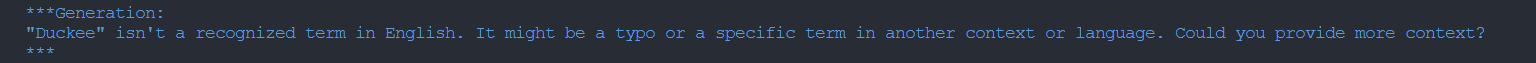
\includegraphics[width=1.0\textwidth, height=0.05\textheight]{IMAGE/hyde_fail.png}
                \caption{Example of HyDE failure case}
                \label{fig:hyde_failure}
            \end{figure}
        \end{itemize}
        \item Performance impact suggests need for more robust hypothetical answer generation strategy
    \end{itemize}
\end{itemize}

% \label{C4} %%%%%%%%%%%%%%%%%%%%%%%%%%%%

%\noindent\rule{\linewidth}{2pt}
%%%%%%%%%%%%%%%%%%%%%%%%%%%%%%%%%%%%%%%%%%%%%%%%%%%%%%%%%%%%%%%%%%%%%%%%%%%%%%%%%%
